\section{Szyfrowanie}

\begin{frame}
	\begin{alertblock}{Szyfrowanie}
		Jest to proces przetwarzania przesyłanej informacji w taki sposób, by była czytelna tylko dla uprawnionych stron komunikacji. Wiadomość zostaje przesłana w zakodowanej postaci, co znacznie utrudnia lub uniemożliwia zrozumienie jej treści w przypadku przechwycenia.
	\end{alertblock}
\end{frame}

\begin{frame}{Szyfrowanie symetryczne}
	Zarówno odbiorca, jak i nadawca dysponują takim samym kluczem.\\
	\vspace{\fill}
	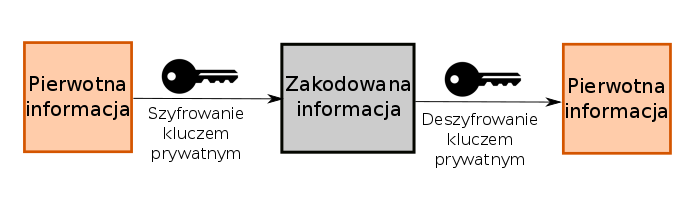
\includegraphics[height=0.25\paperwidth]{images/priv-key.png}
	\vspace{\fill}
	Obie strony muszą znać klucz przed rozpoczęciem komunikacji. Zwiększa to prawdopodobieństwo jego przechwycenia.	
\end{frame}

\begin{frame}{Szyfrowanie asymetryczne}
		\begin{itemize}
			\item Generowane są dwa klucze, prywatny i publiczny.
			\item Klucz publiczny jest ogólnie dostępny.
			\item Utworzenie dwóch takich par eliminuje konieczność wymiany kluczów prywatnych. 
		\end{itemize}	
\end{frame}

\begin{frame}{Szyfrowanie asymetryczne}
		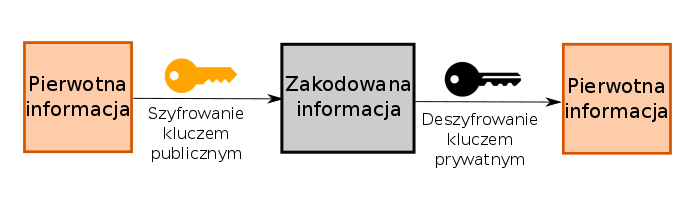
\includegraphics[height=0.25\paperwidth]{images/pub-key.png} \\
		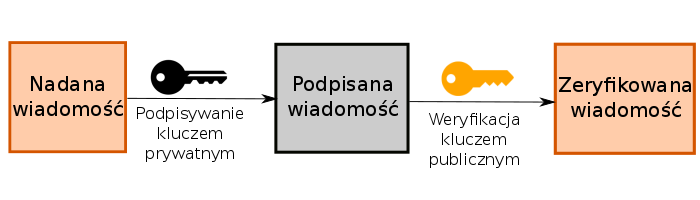
\includegraphics[height=0.25\paperwidth]{images/pub-key-sign.png}
\end{frame}

\begin{frame}{Algorytmy szyfrujące asymetryczne}
	\begin{itemize}
		\item Digital Signature Algorithm (DSA).
		\item ElGamal.
		\item NTRUEncrypt.
		\item Algorytmy bazujące na kryptografii krzywych eliptycznych.
		\item RSA.
	\end{itemize}
\end{frame}

\begin{frame}{Algorytmy szyfrujące symetryczne}
	\begin{itemize}
		\item Advanced Encryption Standard (AES).
		\item Data Encryption Standard (DES).
		\item Blowfish.
		\item IDEA.
		\item RC4.
		\item Tiny Encryption Algorithm.
	\end{itemize}
\end{frame}

\subsection{Protokoły}

\begin{frame}{Protokoły}
	W celu zagwarantowania bezpieczeństwa transmisji danych w sieci, w ustandaryzowanym pakiecie protokołów internetowych wykorzystane szereg metod kryptograficznych.
	\begin{center}
		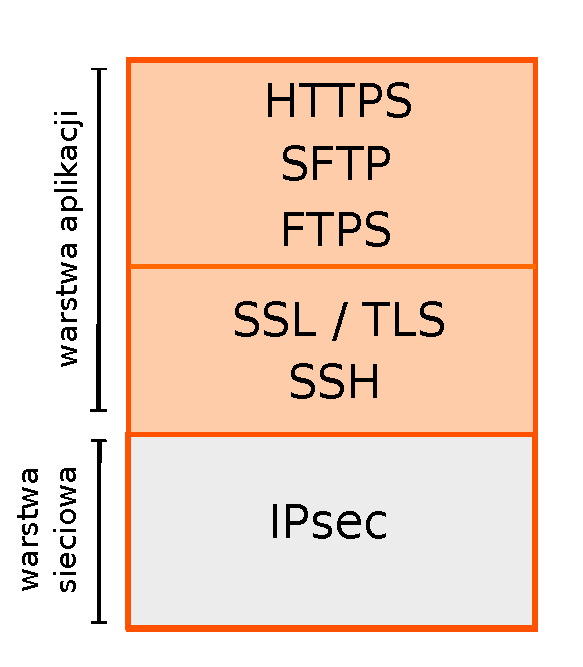
\includegraphics[height=0.4\paperwidth]{images/protocols.pdf}	
	\end{center}

\end{frame}

\begin{frame}{IPsec}
	\begin{alertblock}{Internet Protocol Security}
		Zestaw protokołów wykorzystujących szyfrowanie pakietów i uwierzytelnianie na poziomie warsty sieciowej. 
	\end{alertblock}
		\vspace{\fill}
		Może zostać zaimplementowany w dwóch trybach:
		
		\begin{enumerate}
			\item \textbf{transportowym} — szyfrowane są tylko dane;
			\item \textbf{tunelowym} — szyfrowany jest cały pakiet.
		\end{enumerate}
\end{frame}

\begin{frame}{SSH}
	\begin{alertblock}{Secure Shell}
		Protokół wykorzystujący kryptografię asymetryczną do bezpiecznego zdalnego dostęp do komputera. 
	\end{alertblock}
	
	Połączenie jest realizowane w architekturze klient-serwer. Uwierzytelnienie może zostać przeprowadzone w dwóch wariantach:
	\begin{enumerate}
		\item z automatycznyn generowaniem par kluczy oraz wykorzystaniem hasła;
		\item z ręcznym generowaniem kluczy.
	\end{enumerate}
	
\end{frame}

\begin{frame}{SSH}
	Protokół SSH charakteryzuje się szerokim spektrum zastosowań:
	\begin{itemize}
		\item zdalne wykonywanie komend;
		\item tunelowanie;
		\item przekierowywanie portów TCP;
		\item przekazywanie sesji graficznej X11 (system okien);
		\item przesył plików.
	\end{itemize}
\end{frame}

\begin{frame}{SSL}
	
\end{frame}

\begin{frame}{TSL}
	
\end{frame}

\begin{frame}{HTTPS, SFTP, FTPS}
	
\end{frame}

